\chapter{Background}\label{ch:3}
This chapter mathematically formalizes the problems we consider in this work as well as the algorithms used to solve these problems. We start with the basic definition of a graph and then look at different problems that can be defined on them. Finally, we  

Problems defined on networks arise in many real-life applications. A network can be represented by a graph.

\newcommand{\Ein}[1]{\delta^-(#1)}
\newcommand{\Eout}[1]{\delta^+(#1)}
\newcommand{\ein}{{e_{\text{in}}}}
\newcommand{\eout}{{e_{\text{out}}}}

%for algorithms
%\newcommand{\setfont}[1]{\mathcal{#1}}
\newcommand{\setfont}[1]{#1}

\begin{definition}[directed graph]
A graph is an ordered pair $G = (V, E)$ consisting of a vertex (or node) set $V$ and an edge (or arc) set $E$. In a \textit{directed graph (digraph)}, $E$ is a set of ordered pairs of vertices, a subset of the cartesian product of vertices, that is $E \subseteq V \times V$. Thus, each edge $e \in E$ can be uniquely identified by a pair of vertices from $V$, that is $e=(v,w)$ with $v,w \in V$ and $v \neq w$, where $v$ is the start vertex and $w$ is the end vertex of the directed edge or arc $e$ \cite{jungnickel2013graphs}[1.6]. For problems or algorithms defined on digraphs, it is often convenient to define the sets of edges coming into a vertex $v$ or leaving it.
 E.g. for vertex $v=2$ in \refFigure{fig:graph}, $\Ein{2}=\{(0,2),(1,2)\}, \Eout{2}=\{(2,3)\}$
\begin{align}
\text{incoming edges} \quad \quad \Ein{v}  &: \{ e=(u,v) \in E \; | \; u,v \in V \}  \\
\text{outgoing edges} \quad \quad \Eout{v} &: \{ e=(v,w) \in E \; | \; v,w \in V \}
\end{align}
\end{definition}

\begin{figure}
\centering
	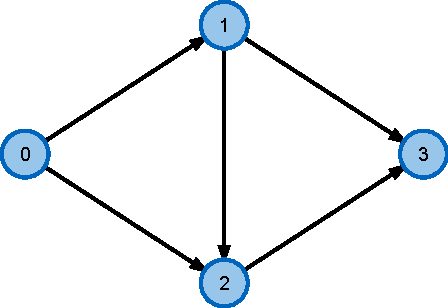
\includegraphics{fig/graph-editor}
	\caption{a digraph with $V=\{0,1,2,3\}$, $E=\{(0,1),(0,2),(1,2),(1,3),(2,3)\}$}
	\label{fig:graph}
\end{figure}



\section{The \maxflow{}}
An important problem in many applications is to find out the maximum amount of flow that can simultaneously be transferred over a network between two points. % from $s$ to $t$. 
Depending on the context, flow can mean different things, e.g the amount of water in a water pipe system in your city or the bandwidth of a computer network. We call such a network a \textit{flow network}:

\begin{definition}[flow network]
A \textit{flow network} $N$ is a 4-tuple $N=(G,c,s,t)$ consisting of \textit{digraph} $G$, a positive real-valued capacity function $c: E \rightarrow \mathbb{R}_+ , \forall e \in E : c(e) \geq 0$ defined on all edges of the graph and two designated vertices, the \textit{source} $s \in V$ and \textit{sink} (or target) $t \in V$ \cite{ahuja1993network}[1.2].
\end{definition}


%However, the links in the network on paths from $s$ to $t$ can only handle flow up to their maximum capacity $c$. One now seeks an assignment of flow values $f$ to edges $e$ that fulfills all the capacity constraints of the edges and the flow conservation property on all the inner nodes, meaning we don't want leaks in our pipe system.
However, the individual links in the network can only handle flow up to their maximum capacity, e.g. they are limited by the thickness of the water pipe. Additionally, the total flow must be preserved at the intermediate joints, e.g. we don't want leaks in our pipe system. This is called a \textit{feasible flow}:% Given such a network, an obvious problem is to find out the maximum amount of flow that can simultaneously be transfered over the network, 


\begin{definition}[feasible flow]
A \textit{feasible flow} $f$ from $s$ to $t$ is a mapping $f : E \rightarrow \mathbb{R}$ satisfying two constraints: The \Eqref{eq:cap} ensures that the flow over an edge is always positive and not exceeding the edge's maximum capacity, while the \Eqref{eq:conserv} assures that the total flow into a vertex $v \notin {s,t}$ equals the total flow out of $v$:
\begin{align}
\forall e \in E &: 0 \leq f(e) \leq c(e) \eqname*[eq:cap]{capacity constraint} \\
\forall v \in V \setminus \{s,t\} &: \sum_{e \in \Ein{v}} f(e) = \sum_{e \in \Eout{v}} f(e) \eqname*[eq:conserv]{flow conservation} \\ \nonumber
\end{align}
\end{definition}

There might be many feasible flows (e.g the zero flow $f = 0 \, \forall e \in E$), but we are especially interested in transferring as much as possible across the network, the \textit{maximum flow}:
\begin{problem}[maximum flow]
A \textit{maximum flow} $\max \abs{f}$ is a \textit{feasible flow} that maximizes the \textit{flow value} $\abs{f}$, the amount of flow which flows from $s$ to $t$. This is the net flow into the sink $t$ or out of the source $s$:
\begin{equation*}
\abs{f} = \sum_{e \in \Ein{t}} f(e) = \sum_{e \in \Eout{s}} f(e)
\end{equation*}
\end{problem}


An important concept in the context of flow algorithms is the residual network capturing possible change to $f$, defined by the residual capacities $c'$ and the \textit{residual graph} $G'$:
\begin{definition}[residual graph]
For a flow $f$ in $G=(V,E)$, we can construct the \textit{residual graph} $G' = (V,E')$ by copying all the vertices $v \in V$ from $G$ and for each $e \in E$ adding one or two edges $e'$ to $E'$ with \textit{residual capacity} $c'$ under the following rules \refFigure{fig:residual}:
\begin{description}
\item[forward edge] if $f(e) < c(e)$ for an edge $e=(a,b) \in E$, then add the forward edge $e' = (a,b)$ with residual capacity $c'(e') = c(e) - f(e)$ to $E'$.
\item[backward edge] if $f(e) > 0$ for an edge $e=(a,b) \in E$, then add the backward edge $e' = (b,a)$ with residual capacity $c'(e') = f(e)$ to $E'$.
\end{description}
\end{definition}

\begin{figure}
\centering
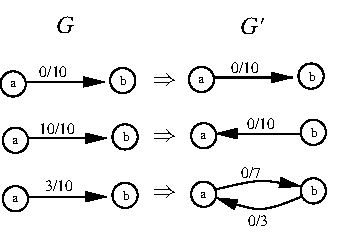
\includegraphics[]{fig/residual}
\caption{Construction of the residual graph $G'$ \cite{mayer2013prakt}.}
\label{fig:residual}
\end{figure}


\section{\pushRelabel{}}
An early way to compute a maximum flow on a directed graph was called the augmenting path method by Ford-Fulkerson \cite{ford1956maximal}. A path with available capacity is an augmenting path, an s-t path in the residual graph. As long as such paths exist, one can increase the flow globally on these paths. If the method terminates, it computed a maximum flow. It is called a method and not an algorithm because the way to find augmenting paths in the residual graph is not fully specified. Furthermore, there is no guarantee on termination and runtime.

About 15 years later, two algorithms based on the augmenting path method were developed. They ensure a polynomial time bound by augmenting flow along the shortest path first. The algorithm of Edmonds-Karp \cite{edmonds1972theoretical} ensures a runtime of $O(|V|\dot|E|^2)$ while the one of Dinic \cite{dinic1970algorithm} improves on that with a runtime of $O(|V|^2\dot|E|)$. This class of algorithms based on the augmenting path method has been visualized in a previous interdisciplinary project \cite{fischer2016idp}.

Still about another 15 years later, an alternative and more efficient method that uses local operations that increase the flow locally was published, the push-relabel algorithm of Goldberg-Tarjan \cite{goldberg1988new}. In contrast to the previous, less efficient algorithms based on augmenting paths, it only changes the flow locally and only needs to construct the residual graph locally. The increased efficiency comes at the cost of not maintaining a \textit{feasible flow} during algorithm execution. Instead, a \textit{preflow} is maintained:
\begin{definition}[preflow]
	The \textit{preflow} $\tilde f$ is a generalization of the flow $f$. The \Eqref{eq:cap} of the edges is still maintained, but the \Eqref{eq:conserv} at the vertices is not: The equality sign $=$ is replaced with $\geq$. This means that more flow can enter an inner node than leaving it, e.g. we allow leaks in our pipe system.
\end{definition}

One allows flow excesses, that is, some vertices can have more incoming than outgoing flow at the intermediate stages of the algorithm \cite{goldberg2014efficient}.

\begin{definition}[excess]
	The \textit{excess} flow at a node $v$ due to the preflow is defined as 
	\begin{align}
		e(v) = \sum_{e \in \Eout{v}} f(e) - \sum_{e \in \Ein{v}} f(e)
	\end{align}
\end{definition}


Another important concept in in the push-relabel algorithm is the height function, which is an approximation of the distance of a node towards the sink. The local \textit{push} operations try to move \textit{excess} at inner nodes 'downwards' towards the sink. If the current node is at a local minimum and still has excess, we \textit{relabel} the node by increasing its \textit{height} so that subsequent push operations can remove the excess.
\begin{definition}[valid edge with respect to the height function]
	An edge $e'=(v,w)$ of the \textbf{residual graph} is valid with respect to the current height function, if $h(v)==h(w)+1$, meaning that the current node is one level above the one to where we wish to push excess to.
\end{definition}

The important property of the push-relabel algorithm is that when the algorithm terminates, the computed preflow is actually a flow!

\documentclass[a4paper,11pt]{article}

\usepackage[linesnumbered,ruled,vlined]{algorithm2e}
%\newcommand{\setfont}[1]{\mathcal{#1}}
\newcommand{\setfont}[1]{#1}

\begin{document}

\begin{algorithm}[h!]
\caption{Goldberg-Tarjan Push-Relabel algorithm}
\DontPrintSemicolon % Some LaTeX compilers require you to use \dontprintsemicolon instead
\KwIn{directed Graph $G=(V,E)$ with
\begin{itemize}
	\setlength\itemsep{0pt}
	\setlength{\parskip}{0pt}
	\item digraph $G=(V,E)$ with start $s$, sink $t$
	\item $\forall$ edges $e \in E$: (cap) capacity 
\end{itemize}
}
\KwOut{A feasible maximum s-t flow f(e)}\vspace{0.2cm}
(* Initialize the preflow *)\;
\ForAll{$e=(u,w) \in E$}{
	\If{$u==s$}{
		$f(e) \gets c(e)$\;
		\If{$w \neq t$}{$Q$.add(w)}
	}
	\Else{$f(e) \gets 0$}
}
((* Initialize the height function *))\;
$h(s) = |V|$\;
\ForAll{$v \in V$}{
	$h(v) \gets$ number of arcs on directed v-t path\;
}
((* Main Loop *))\;
\While{$\setfont{Q} \neq \emptyset$}{
	$v \gets \setfont{Q}$.pop()\;
	\While{$e(v)>0$ AND $\exists e'=(v,w) \in E' | h(v)==h(w)+1$}{
		(* Push *)\;
		push $\min(e(v),c'(e'))$ flow from v to w\;
		\If{$w \neq s,t$ AND $w \notin \setfont{Q}$}{
			$\setfont{Q}$.add($w$)\;
		}
	}
	\If{$e(v)>0$ AND $\not\exists e'=(v,w) \in E' | h(v)==h(w)+1$}{
		(* Relabel *)\;
		$h(v) \gets 1 + \min(h(w) | e*=(v,w)\in E'$ \;
		$\setfont{Q}$.add($v$) \;
	}
}
\end{algorithm}


\end{document}


\section{concept}
\begin{figure}
\centering
\begin{subfigure}[t]{0.45\textwidth}
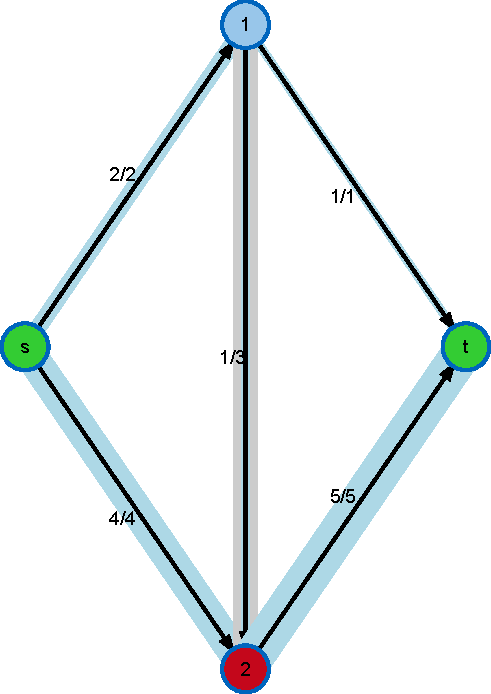
\includegraphics[width=\textwidth]{fig/maxflow-graph-algorithm-graph}
\end{subfigure}
\begin{subfigure}[t]{0.45\textwidth}
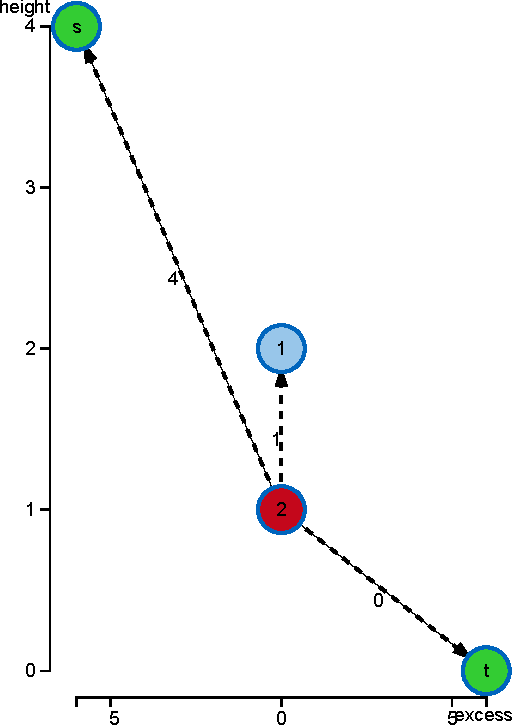
\includegraphics[width=\textwidth]{fig/maxflow-graph-algorithm-height}
\end{subfigure}
\caption{maxflow concept}
\label{fig:maxflow}
\end{figure}


The crucial requirement is the third one, namely d(v) = d(w) + 1. Thus we are only allowed to push along residual edges vw for which d(v) is exactly one unit larger than d(w), that is, for which d(v) takes its maximum permissible value; see (5) above. We may visualize this rule by thinking of water cascading down a series of terraces of different height, with the height corresponding to the labels. Obviously, water will flow down, and condition (5) has the effect of restricting the layout of the terraces so that the water may flow down only one level in each step. \cite{jungnickel2013graphs,6.6}



\section{The \spprc{}}
Another basic problem defined on networks is how to traverse a network to get from one point to another one as cheaply as possible. For this problem we wish to find a shortest path between two points.

\begin{definition}[path]
A \textit{path} $P = (e_1, e_2, ... e_p)$ is a finite sequence of arcs (some arcs may occur more than once) where the end vertex of $e_i \in E$ is identical to the start vertex of $e_{i+1} \in E$ for all $i=1,\dots,p-1$. For simple graphs, a path can be also be written as $P = (v_0,v_1,\dots,v_p)$ since the edges can be uniquely idetified by start and end vertex $e_i=(v_{i-1},v_i)$. The length of a path is $p$ \cite{irnich2005shortest}.
\end{definition}


The ordinary shortest path problem (SPP) is perhaps the simplest of all network problems. It seeks an (unconstrained) $s$-$t$ path of minimal cost (or length) between two points. A real-valued cost function $c : E \rightarrow \mathbb{R}$ is defined on all edges of the graph. The cost or length of a path is defined as the sum of the costs of all the edges along the path, that is $c(P)=\sum_{i=1}^p c(e_i)$. \\



In the shortest path problem with resource constraints (SPPRC), each edge additionally carries a secondary (possibly higher-dimensional) resource vector or function $r$. A path $P$ is now constrained at the intermediate vertices $v_i$ with lower and upper bounds on the accumulated resource consumptions along the (partial) paths.\\

\begin{example}[SPPTW]
An illustrative example is the two-resource SPPRC, the shortest path problem with time windows (SPPTW). In addition to the \textit{cost} $c$, each edge additionally bears the resource \textit{time} $t$. Thus each edge is associated with the two-dimensional resource vector $(t,c) \forall e \in E$. The secondary resource \textit{time} is constrained, while the primary resource \textit{cost} is unconstrained, but seeks to be minimized.

The accumulated consumptions of the resource \textit{time} along a path are constrained at the intermediate vertices along that path by lower and upper limits, that is the earliest arrival time $t_a$ and the latest departure time $t_b$ and called the \textit{resource window}, denoted as tuples $[t_a,t_b] \, \forall v \in V$.
\end{example}



\section{\labelSetting{}}
%\documentclass[a4paper,11pt]{article}
%\usepackage[linesnumbered,ruled,vlined]{algorithm2e}
%%\newcommand{\setfont}[1]{\mathcal{#1}}
%\newcommand{\setfont}[1]{#1}
%\begin{document}

\begin{algorithm}[h!]
\DontPrintSemicolon % Some LaTeX compilers require you to use \dontprintsemicolon instead
\KwIn{directed Graph $G=(V,E)$ with
\begin{itemize}
	\setlength\itemsep{0pt}
	\setlength{\parskip}{0pt}
	\item $\forall$ nodes $v \in V$: [arrive, depart] time window resource constraint
	\item $\forall$ edges $e \in E$: (time,cost) 2-dimensional resource consumptions
	\item start Node $s$, end Node $t$
\end{itemize}}
\KwOut{feasible, pareto-optimal $s \rightarrow t$ paths} \vspace{0.2cm}
(* Initialize *) \;
SET $\setfont{U} = \{(s)\}$ and $\setfont{P} = \emptyset$ \;
\While{$\setfont{U} \neq \emptyset$}{
	(* Path extension step *)\;
	CHOOSE a path $\setfont{Q} \in \setfont{U}$ and REMOVE $\setfont{Q}$ from $\setfont{U}$\;
	\ForAll{arcs $(v(\setfont{Q}), w) \in A$ of the forward star of $v(\setfont{Q})$}{
		\If{$(\setfont{Q},w) \in \setfont{F}(s,w) \cap \setfont{G}$}{
			ADD $(\setfont{Q},w)$ to $\setfont{U}$
		}
	}
	ADD $\setfont{Q}$ to $\setfont{P}$\;
	(* Dominance step *)\;
	\If{(* any condition *)}{
		APPLY dominance algorithm to paths from $\setfont{U} \cup \setfont{P}$ ending at some node $v$\;
	}
}
(* Filtering step *)\;
FILTER $\setfont{P}$, i.e., identify a solution $\setfont{S} \subseteq \setfont{P}$\;
\caption{Generic Dynamic Programming SPPRC Algorithm}
\end{algorithm}


%\end{document}


\section{concept}

\begin{figure}
\centering
\begin{subfigure}[t]{0.45\textwidth}
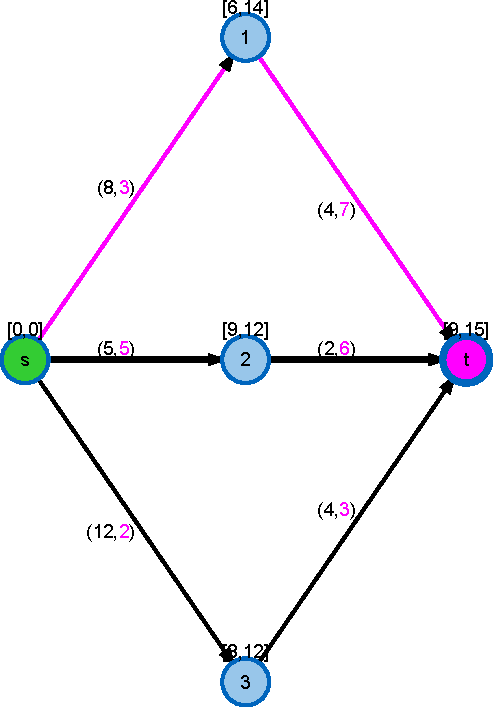
\includegraphics[width=\textwidth]{fig/spp-rc-graph-algorithm-graph}
\end{subfigure}
\begin{subfigure}[t]{0.45\textwidth}
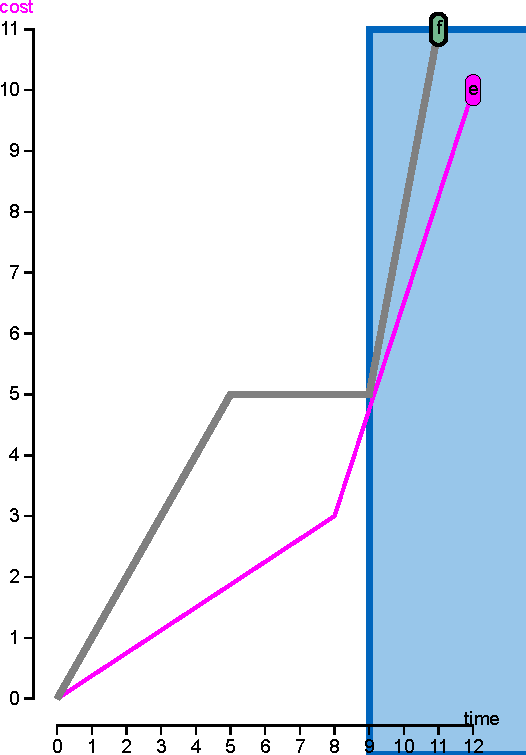
\includegraphics[width=\textwidth]{fig/spp-rc-graph-algorithm-labels}
\end{subfigure}
\caption{spprc concept}
\label{fig:spprc}
\end{figure}


